\فصل{راه‌حل پیشنهادی}

برای درک بهتر موضوع همزمان با توضیح راه‌حل یک مثال را به طور موازی پیش می‌بریم.
هدف از این رساله بیان راه‌حلی برای پیش‌بینی سرعت ترافیک در برخی مختصات‌ها (مانند تعدادی میدان) در چند گام زمانی آینده است که
بدین جهت از سرعت ترافیک در این محل‌ها در گام‌های زمانی پیشین استفاده می‌کنیم. رابطه \رجوع{eq:base} این مساله سری زمانی را به زبان ریاضی توصیف می‌کند.

\begin{equation}
  \label{eq:base}
  \hat{v}_{t+1}, \ldots,  \hat{v}_{t+H} = \mathop{\mathrm{argmax}} \log \mathsf{P}({v}_{t+1}, \ldots,  v_{t+H} | v_{t-M+1} , \ldots,  v_{t})
\end{equation}

\begin{table}[h]
  \centering
  \caption{توضیح پارامترهای رابطه \رجوع{eq:base}}
  \begin{tabular}{|c|p{0.5\textwidth}|}
    \hline
    $v_{t}$ & یک بردار به طول تعداد نقاطی که قصد داریم سرعت ترافیک را در آن‌ها پیش‌بینی کنیم که هر المان شامل سرعت ترافیک در یکی از مختصات‌های مورد نظر در زمان $t$ است. \\
    \hline
    $\hat{v}_{t+1}$ & سرعت پیش‌بینی شده در زمان $t+1$ \\
    \hline
    $H$ & تعداد گام های زمانی آینده که می‌خواهیم سرعت ترافیک را پیش بینی کنیم. \\
    \hline
    $M$ & تعداد گام های زمانی پیشین که برای پیش بینی استفاده می‌کنیم. \\
    \hline
  \end{tabular}
  \label{tbl:base}
\end{table}

برای مثال فرض کنیم می‌خواهیم سرعت ترافیک را در میدان فاطمی و میدان فلسطین (دو میدان معروف در تهران) پیش‌بینی کنیم.
$v_{t}$ یک بردار به طول دو خواهد بود که یک عضو آن سرعت ترافیک در میدان فاطمی در زمان $t$ مانند ساعت دو بعد از ظهر امروز و عضو دیگر آن شامل همین اطلاعات برای میدان فلسطین خواهد بود.
در این مثال $H$ را برابر یک و $M$ را برابر سه در نظر می‌گیریم. منظور از \رجوع{eq:base} این است که قصد داریم سرعت ترافیک در $H$ قدم زمانی بعدی را با دانستن $M$ قدم زمانی قبلی پیش‌بینی کنیم.

برای پیش‌بینی سرعت ترافیک در نقاط مختلف از هر دو نوع ویژگی زمانی و مکانی بهره می‌بریم.
در روش‌های پیشین مانند \مرجع{1506.04214} از پیچش\پانویس{convolution} معمول که عمدتا در پردازش تصویر از آن بهره می‌گیرند استفاده شده است، این پیچش تنها می‌تواند بر روی داده‌هایی اعمال شود که ساختار مشبک دارند (مانند عکس و فیلم).
در این روش برای آنکه بتوانیم از اطلاعات مکانی حداکثر استفاده را ببریم به جای آنکه شبکه‌ی ترافیک را مانند یک شبکه‌‌ی شطرنجی\پانویس{Grid} ببینیم،
آن را به وسیله‌ی یک گراف مدل می‌کنیم و پیچش را مستقیما بر روی این گراف اعمال می‌کنیم.

گره‌های این گراف نقاطی مشخص هستند که سرعت ترافیک را در آن‌ها داشته باشیم، در این مثال نقاط ما میدان‌های فاطمی و فلسطین هستند،
سرعت در این نقاط به طور مثال می‌تواند از طریق دوربین‌های سرعت سنج یا از طریق سیستم موقعیت‌‌یاب‌جهانی\پانویس{GPS} رانندگان تشخیص داده شود.

\begin{figure}
  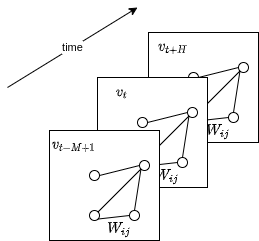
\includegraphics{./images/base.png}
  \centering
  \caption{
نمایش رابطه \رجوع{eq:base} به صورت شهودی.
گراف مسیر یکسان است و هر دیاگرام نشان‌دهنده‌ی سرعت ترافیک در گره‌های این گراف در یک لحظه متفاوت است.
}
  \label{fig:base}
\end{figure}

بدیهی است تغییر سرعت ترافیک در یک گره‌ی گراف می‌تواند باعث تغییر سرعت ترافیک در گره‌های مجاور شود و هر چه فاصله‌ی دو گره از یک دیگر کم تر باشد این اثرگذاری قوی‌تر است.
برای نمایش این عامل به صورت کمی از ماتریس $W$ استفاده می‌کنیم، ابعاد این ماتریس به صورت $n \times n$ است که $n$ برابر تعداد گره‌های گراف است و هر مقدار داخل این ماتریس تابعی از فاصله‌ی بین دو گره متناظر است که مقدار آن با کاهش این فاصله بیشتر می‌شود.

در شکل \رجوع{fig:base} $W_{i,j}$ مقدار ماتریس $W$ در خانه‌ی $i$ و $j$ است که نشان دهنده‌ی میزان ارتباط مکانی و همبستگی بین گره‌های $i$ و $j$ می‌باشد.
در این مثال گره‌های $i$ و $j$ همان میادین یاد شده هستند و $W_{i,j}$ با توجه به فاصله‌ی مکانی این دو میدان نشان می‌دهد که
به طور مثال اگر سرعت ترافیک در میدان فاطمی کاهش پیدا کند این موضوع چقدر می‌تواند بر روی سرعت ترافیک در میدان فلسطین تاثیر بگذارد.
در این پروژه از رابطه‌ \رجوع{eq:distance} برای بدست آوردن خانه‌های ماتریس $W$ استفاده می‌کنیم \مرجع{1709.04875}:

\begin{equation}
  W_{i,j} = \left\{
    \begin{array}{ll}
      \exp(-\frac{d^{2}_{ij}}{\sigma^{2}}) & , i \neq j \quad and \quad \exp(-\frac{d^{2}_{ij}}{\sigma^{2}}) \geq \epsilon \\
      0 & , otherwise. \\
    \end{array}\right.
  \label{eq:distance}
\end{equation}

\begin{table}[h]
  \centering
  \caption{توضیح پارامترهای رابطه \رجوع{eq:distance}}
  \begin{tabular}{|c|p{0.5\textwidth}|}
    \hline
    $W_{ij}$ & میزان ارتباط مکانی بین گره‌های $i$ و $j$ \\
    \hline
    $d_{ij}$ & فاصله ی مکانی بین گره‌های $i$ و $j$ \\
    \hline
    $\sigma$, $\epsilon$ & پارامترهای ثابت برای کنترل میزان تنک\پانویس{Sparsity} بودن ماتریس $W$ \\
    \hline
  \end{tabular}
  \label{tbl:distance}
\end{table}

در مثال ما فاصله بین میدان‌های فاطمی و فلسطین برابر $1.7$ کیلومتر است.
هرچه $\epsilon$ را افزایش دهیم باعث می‌شود تنها ارتباطات قوی‌تر را به حساب بیاوریم و ماتریس تنک‌تر می‌شود
همچنین هرچه $\sigma$ را کاهش دهیم عددی که به عنوان میزان ارتباط محاسبه می‌کنیم کاهش یافته و ماتریس تنک‌تر می‌شود.

با توجه به توضیحات بالا برنامه توسعه‌یافته‌ی نهایی بر اساس این مدل برای عملکرد به دو فایل ورودی احتیاج دارد که اطلاعات درج شده در شکل \رجوع{fig:blackbox} را در اختیار برنامه قرار دهند.
فایل اول شامل ماتریس $W$ است که پیشتر توضیح داده شد و گراف یا به عبارتی وزن یال‌ها را شرح می‌دهد،
فایل دیگر شامل سرعت ترافیک در نودهای این گراف در بازه‌های زمانی متوالی قرار می‌گیرد $(V_{t}, \ldots, V_{t-M+1})$.
در خروجی، سرعت ترافیک پیش‌بینی شده در نودها در قدم‌های زمانی بعدی برگردانده می‌شود $\hat{V}$.
در مثال ما فایل‌های ذکر شده فرمتی مانند جدول \رجوع{tbl:speed-example} و \رجوع{tbl:distance-example} دارند البته اعداد زیر به صورت تصادفی و فرضی هستند.

\begin{figure}
  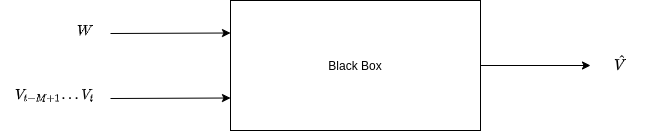
\includegraphics[height=3cm]{./images/blackbox.png}
  \centering
  \caption{
در یک نگاه سطح بالا برنامه با دانستن گراف و سرعت ترافیک در گره‌های این گراف در $M$ واحد زمانی گذشته سرعت ترافیک در $H$ واحد زمانی بعدی را تخمین زده و برمی‌گرداند.
  }
  \label{fig:blackbox}
\end{figure}

\شروع{لوح}[h]
\شرح{مثالی از فرمت فایل ورودی برنامه که شامل سرعت ترافیک در میادین فلسطین و فاطمی در سه قدم زمانی است.}
\تنظیم‌ازوسط
\برچسب{tbl:speed-example}
\شروع{جدول}{|c|c|c|c|}
\خط‌پر
۲ بعد از ظهر & ۱:۵۵ بعد از ظهر & ۱:۵۰ بعد از ظهر & \\
\خط‌پر
۳۶ کیلومتر بر ساعت & ۳۲ کیلومتر بر ساعت & ۴۰ کیلومتر بر ساعت & میدان فلسطین \\
\خط‌پر
۱۷ کیلومتر بر ساعت & ۲۷ کیلومتر بر ساعت & ۱۰ کیلومتر بر ساعت & میدان فاطمی \\
\خط‌پر
\پایان{جدول}
\پایان{لوح}

\شروع{لوح}[h]
\شرح{مثالی از فرمت فایل ورودی برنامه که شامل وزن یالها برای نشان دادن میزان ارتباط مکانی است.}
\تنظیم‌ازوسط
\برچسب{tbl:distance-example}
\شروع{جدول}{|c|c|c|}
\خط‌پر
میدان فاطمی & میدان فلسطین & \\
\خط‌پر
۳۱۶ & ۰ & میدان فلسطین \\
\خط‌پر
۰ & ۳۱۶ & میدان فاطمی \\
\خط‌پر
\پایان{جدول}
\پایان{لوح}


برای سادگی گراف را بدون جهت در نظر می‌گیریم و در نتیجه $W$ ماتریسی متقارن است.

برنامه برای آنکه بتواند هم ارتباطات مکانی و هم ارتباطات زمانی را یاد بگیرد باید از بلوک‌هایی تشکیل شده باشد که هر دو نوع لایه پیچشی زمانی و مکانی را در خود داشته باشند.
همانطور که در شکل \رجوع{fig:blocks} نشان داده شده است، ساختار برنامه از دو بلوک پیچشی زمانی-مکانی و یک لایه‌ی خروجی کاملا متصل در انتها تشکیل شده است.

\begin{figure}
  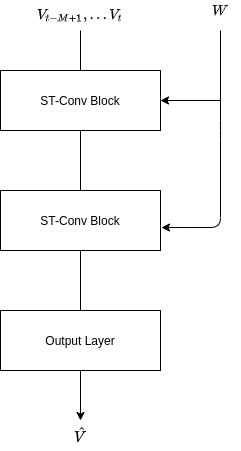
\includegraphics[height=8cm]{./images/blocks.png}
  \centering
  \caption{
شبکه‌ی پیچشی زمانی-مکانی بر روی گراف \مرجع{1709.04875}
  }
  \label{fig:blocks}
\end{figure}

هر بلوک پیچشی زمانی-مکانی که در شکل \رجوع{fig:inner-blocks} نشان داده شده است از دو لایه‌ی پیچشی زمانی تشکیل شده است که در ورودی و خروجی قرار گرفته‌اند
و یک لایه‌ی پیچش مکانی گراف مانند پلی بین آن دو قرار گرفته است، که می‌تواند با سرعت خوبی اطلاعات مکانی را پس از اعمال پیچش روی گراف
به پیچش‌های زمانی انتشار دهد.

\begin{figure}
  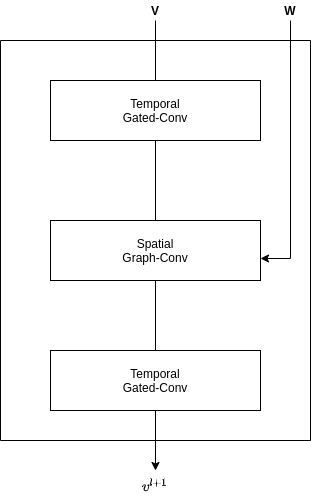
\includegraphics[height=8cm]{./images/inner-blocks.png}
  \centering
  \caption{
ساختار بلوک پیچشی زمانی-مکانی. گراف مسیرها تنها در لایه‌ی پیچش مکانی گراف استفاده می‌شود. \مرجع{1709.04875}
  }
  \label{fig:inner-blocks}
\end{figure}

در این پروژه برای استخراج ویژگی‌های مکانی از پیچش روی گراف استفاده می‌کنیم و بدیهی است پیچش استاندارد که معمولا
در بحث پردازش تصویر روی تصاویر اعمال می‌کنیم در این مساله قابل استفاده نیست
چرا که در پردازش تصویر پیچش عملا کار الگویابی\پانویس{Pattern Matching} را انجام می‌دهد اما در گراف که رئوس جای مشخصی ندارد
و راس‌های یک گراف را می‌توان به صورت‌های مختلفی
شماره‌گذاری کرد نمی‌توان از پیچش انتظار الگویابی داشت.
و باید از مدل عمومی‌تری استفاده کنیم.

در پردازش تصویر از کرنل‌هایی مانند شکل \رجوع{fig:2d-convolution} استفاده می‌شود. تمامی خانه‌ها همواره در جای مشخص خود و با ترتیب ثابت قرار گرفته‌اند
برای مثال خانه‌ی $j3$ همیشه در گوشه بالا قرار گرفته است.

\begin{figure}
  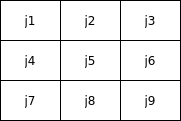
\includegraphics[]{./images/2d-convolution.png}
  \centering
  \caption{کرنل پیچش دو بعدی}
  \label{fig:2d-convolution}
\end{figure}

می‌خواهیم کرنل شکل \رجوع{fig:graph-convolution-kernel}
به گراف شکل \رجوع{fig:graph-convolution-graph} اعمال کنیم و واضح است که یک نام‌گذاری با ترتیب یکسان برای گراف و کرنل وجود ندارد.


\begin{figure}
  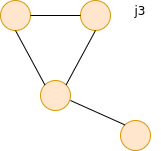
\includegraphics[]{./images/graph-convolution-kernel.png}
  \centering
  \caption{کرنل پیچش گراف}
  \label{fig:graph-convolution-kernel}
\end{figure}

\begin{figure}
  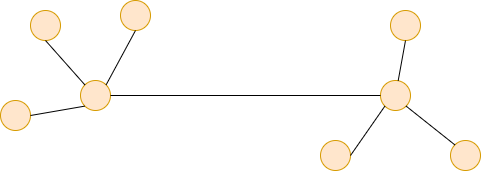
\includegraphics[]{./images/graph-convolution-graph.png}
  \centering
  \caption{گراف مقصد پیچش گراف}
  \label{fig:graph-convolution-graph}
\end{figure}

در این پژوهش از پیچش طیفی روی گراف‌\پانویس{Spectral Graph Convolution} استفاده می‌کنیم. \مرجع{1312.6203}

با استفاده از رابطه \رجوع{eq:convolution} می‌توانیم پیچش روی گراف را انجام دهیم تا الگوها و ویژگی‌های با معنی را در دامنه‌ی فضا پیدا کنیم.

\begin{equation}
  \Theta *_{g} \chi = \Theta(L)\chi = \Theta(U \Lambda U^{T})\chi = U\Theta(\Lambda)U^{T}\chi
  \label{eq:convolution}
\end{equation}

\begin{table}[h]
  \centering
  \caption{توضیح پارامترهای رابطه \رجوع{eq:convolution}}
  \begin{tabular}{|c|p{0.5\textwidth}|}
    \hline
    $*_{g}$ & عامل پیچش مکانی روی گراف \\
    \hline
    $\chi$ & سیگنال گراف که در این مدل خروجی لایه‌ی پیچش زمانی اول است \\
    \hline
    $\Theta$ & کرنل \\
    \hline
    $L$ & ماتریس لاپلاسین نرمال شده‌ی گراف \\
    \hline
    $U$ & ماتریس بردار ویژه‌های ماتریس $L$ \\
    \hline
    $\Lambda$ & ماتریس قطری مقدار ویژه‌های ماتریس $L$ \\
    \hline
  \end{tabular}
  \label{tbl:distance}
\end{table}

در مثال ذکر شده اگر محاسبات را انجام دهیم، خواهیم داشت:

\[
U = \left(
  \begin{array}{cc}
  1 & -1 \\
  1 & 1 \\
  \end{array}
\right),
\Lambda = \left(
  \begin{array}{cc}
  0 & 0 \\
  0 & 2 \\
  \end{array}
\right),
L = \left(
  \begin{array}{cc}
  1 & -1 \\
  -1 & 1 \\
  \end{array}
\right)
\]

در نظر داشته باشید که المان‌های ماتریس $\Theta$ در ابتدا به صورت تصادفی انتخاب می‌شوند.

پیچیدگی زمانی این رابطه $O(n^{2})$ است که بسیار سنگین است، برای سبک شدن محاسبات باید از یک تخمین به جای استفاده مستقیم از این رابطه بهره ببریم.
در این پروژه از تخمین چند جمله‌ای چبیشف\پانویس{Chebyshev} استفاده می‌کنیم.

برای متمرکز و محلی کردن فیلتر و کاهش تعداد پارامترها، می‌توان کرنل $\Theta$ را به یک چند جمله‌ای از $\varLambda$ محدود کرد.

\[
  \Theta(\varLambda) = \sum_{k=1}^{k-1}\Theta_{k}\varLambda^{k}
\]

$k$ اندازه کرنل در پیچش گراف است که شعاع بیشینه پیچش از یک گره مرکزی را مشخص می‌کند. از چند جمله‌ای چبیشف $T_{k}(x)$ استفاده می‌کنیم تا
کرنل‌ها را به صورت انبساطی کوتاه شده از مرتبه‌ی $k-1$ تخمین بزنیم.

 از چند جمله‌ای چبیشف
( $T_{k}(x)$ )
 استفاده می‌کنیم تا کرنل‌ها را به صورت انبساطی کوتاه شده از مرتبه‌ی
 $k-1$
 تخمین بزنیم.

\[
  \Theta(\varLambda) \approx \sum_{k=1}^{k-1}\Theta_{k}T_{k}(\widetilde{\varLambda})
\]
\[
  \widetilde{\varLambda} = \frac{2\varLambda}{\lambda_{\max}} - I_{n}
\]

% \begin{table}[h]
%   \centering
%   \caption{توضیح پارامترهای رابطه \رجوع{eq:convolution}}
%   \begin{tabular}{|c|p{0.5\textwidth}|}
%     \hline
%     $\Lambda$ & ماتریس قطری مقدار ویژه‌های ماتریس $L$ \\
%     \hline
%     $\lambda_{\max}$
%     & بزرگ‌ترین مقدار ویژه‌ی ماتریس لاپلاسین \\
%     \hline
%     $\Theta$ & کرنل \\
%     \hline
%     $L$ & ماتریس لاپلاسین نرمال شده‌ی گراف \\
%     \hline
%     $U$ & ماتریس بردار ویژه‌های ماتریس $L$ \\
%     \hline
%     $\widetilde{\varLambda}$
%     & $\varLambda$ اسکیل شده \\
%     \hline
%   \end{tabular}
%   \label{tbl:distance}
% \end{table}

حال می‌توانیم پیچش روی گراف را اینگونه بازنویسی کنیم:

\begin{equation}
  \Theta \ast_{g} x = \Theta(L)x \approx \sum_{k=0}^{k-1} \Theta_{k} T_{k}(\widetilde{L})x
  \label{eq:approx-convolution}
\end{equation}

$T_{k}(\widetilde{L} \in R^{n \times n})$ چند جمله‌ای چبیشف از مرتبه‌ی $k$ است که به وسیله‌ی لاپلاسین اسکیل شده محاسبه می‌شود.

\[
  \widetilde{L} = \frac{2\widetilde{L}}{\lambda_{\max}} - I_{n}
\]

از تقریب چند جمله‌ای استفاده می‌کنیم و به طور بازگشتی $k$ پیچش‌های محلی را محاسبه می‌کنیم. اینگونه می‌توانیم رابطه‌ی \رجوع{eq:convolution}
را با رابطه‌ی \رجوع{eq:approx-convolution} تخمین بزنیم و پیچیدگی محاسباتی را از $O(n^{2})$ به $O(k|\epsilon|)$
کاهش دهیم.

\زیرقسمت{تعمیم دادن کانولوشن روی گراف}
\پاراگراف{}
عامل کانولوشن بر روی گراف (
$*_g$
)که پیشتر تعریف کردیم تنها می توانست بر روی یک
$x \in R^n$
اعمال شود. می توانیم آن را تعمیم دهیم به طوری که بر روی تنسورهای چندبعدی نیز قابل اعمال باشد. برای سیگنالی با
$c_i$
کانال (
$X \in R^{n*c_i}$
)
کانولوشن روی گراف را می توان اینگونه تعمیم داد

\begin{equation}
y_i = \sum_{i=1}^{C_i} \Theta _{i,j}(L)x_i \in R^n , 1 <= j <= C_o
    \label{eq:graph-convolution-generalization}
\end{equation}

\begin{table}[h]
  \centering
  \caption{توضیح پارامترهای رابطه \رجوع{eq:graph-convolution-generalization}}
  \begin{tabular}{|c|p{0.5\textwidth}|}
    \hline
    $C_i$ & سایز ورودی نگاشت ویژگی\پانویس{feature map} \\
    \hline
    $C_o$ & سایز خروجی نگاشت ویژگی \\
    \hline
    $\Theta_{i,j} \in R^k$ & بردارهای ضرایب چبیشف که تعداد آن‌ها
    $C_i * C_o$
    می‌شود.\\
    \hline
  \end{tabular}
  \label{tbl:distance}
\end{table}

\پاراگراف{}
کانولوشن بر روی گراف برای متغیرهای دو بعدی به صورت
$\Theta *_g X$
نشان داده می‌شود (
$\Theta \in R^{K*C_i*C_o}$
. در این پروژه برای پیش‌بینی ترافیک ورودی از
$M$
صفحه تشکیل شده‌است که هر صفحه گراف مسیرها را در یک گام زمانی نشان می‌دهد ( شکل
\رجوع{fig:base}
).
هر صفحه مربوط به گام زمانی
$t$
را می توان به صورت یک ماتریس دید که ستون
$i$
ام آن مقدار
$C_i$
بعدی از سرعت ترافیک در گره
$i$
ام از گراف است (
$X \in R^{n * C_i}$
)

\پاراگراف{}
در مسائل سری زمانی، شبکه‌های عصبی بازگشتی بسیار رایج‌اند اما در مسایل ترافیک استفاده از این شبکه‌ها بسیار زمان‌بر است.
همچنین در ترافیک تغییرات به صورت پویا می‌باشند که این شبکه دیر به این تغییرات جواب می‌دهد،
در طرف دیگر شبکه های عصبی پیچشی به سرعت آموزش داده می‌شوند و ساختار ساده‌ای دارند، در نتیجه برای استخراج ویژگی‌های زمانی در این پروژه با الهام از
\مرجع{1409.3215} از ساختارهای کاملا پیچشی بر روی محور زمان استفاده می‌کنیم تا بتوانیم رفتار پویای سرعت ترافیک را دنبال کنیم.

\begin{figure}
  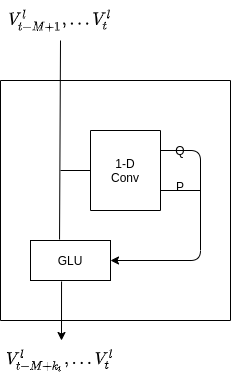
\includegraphics[height=8cm]{./images/time-conv.png}
  \centering
  \caption{
ساختار لایه‌ی کانولوشنی زمانی \مرجع{1709.04875}
  }
  \label{fig:time-conv}
\end{figure}

\پاراگراف{}
شکل \رجوع{fig:time-conv} لایه‌ی پیچشی زمانی را نشان می‌دهد که شامل یک پیچش علّی یک بعدی\پانویس{1-D casual convolution}
با یک فیلتر به عرض  $k_{t}$ است که پس از آن یک \متن‌لاتین{Gated Linear Unit} قرار دارد.
برای هر گره در گراف $g$ پیچش زمانی بر روی تمامی $K_{t}$ همسایه‌ی ورودی اعمال می‌شود.
در این پیچش لایه گذاری\پانویس{padding} وجود ندارد‌‌، در نتیجه، پیچش در هر مرتبه باعث کوتاه‌تر شدن توالی‌ها به اندازه‌ی $K_{t}-1$ می‌شود.
با این توضیحات می‌توانیم رابطه‌ی \رجوع{eq:time-conv} را بیان کنیم.

\begin{equation}
  \Gamma *_{\tau} Y = P \odot \sigma (Q) \in R^{M-K_{t}+1 \times C_{O}}
  \label{eq:time-conv}
\end{equation}

\begin{table}[h]
  \centering
  \caption{توضیح پارامترهای رابطه \رجوع{eq:time-conv}}
  \begin{tabular}{|c|p{0.5\textwidth}|}
    \hline
    $*_{g}$ & عامل پیچش زمانی \\
    \hline
    $Y$ & سرعت ترافیک در گره‌های مختلف گراف در گام‌های زمانی گذشته \\
    \hline
    $\Gamma$ & کرنل پیچش که المان‌های آن در ابتدا به صورت تصادفی انتخاب می‌شوند. \\
    \hline
    $P$, $Q$ & پس از آنکه با استفاده از کرنل $\Gamma$ یک پیچش روی $Y$ اعمال کردیم خروجی را برحسب سایز کانال خروجی لایه به دو نیمه‌ی مساوی تقسیم می‌کنیم که یکی $P$ و دیگری را $Q$ می‌نامیم. \\
    \hline
    $\odot$ & نمایشگر عملیات ضرب درایه‌ای \\
    \hline
    $M$ & تعداد گام‌های زمانی استفاده شده برای آموزش \\
    \hline
    $K_{t}$ & سایز کرنل \\
    \hline
    $C_{O}$ & سایز کانال خروجی \\
    \hline
  \end{tabular}
  \label{tbl:distance}
\end{table}

 $P$ و $Q$ پس از محاسبه به عنوان ورودی به \متن‌لاتین{Gated Linear Unit} داده می‌شوند، این واحد باعث غیرخطی شدن محاسبات این لایه می‌شود.

ورودی $Y$ چهار بعدی است، بُعد اول برابر تعداد کل داده‌هایی است که در اختیار داریم، بُعد دوم برابر
تعداد گام‌های گذشته است، که قصد داریم برای پیش‌بینی استفاده کنیم،
بُعد سوم برابر تعداد گره‌های گراف و در نهایت بُعد آخر سایز کانال ورودی است.
در مثالی که با آن پیش می‌رویم تعداد کل داده‌ها سه، تعداد گام‌های زمانی گذشته مورد استفاده برای پیش‌بینی مدل برابر دو،
تعداد گره‌های گراف برابر دو و سایز کانال ورودی برابر یک است، در نتیجه ابعاد $Y$ به صورت $ 3 \times 2 \times 2 \times 1 $ در میاید.

همانطور که پیش‌تر اشاره شد در این پیچش لایه‌گذاری وجود ندارد در نتیجه ابعاد خروجی این لایه مانند ابعاد ورودی است به جز بعد دوم
که پس اعمال پیچش به اندازه‌ی $K_{t}-1$ کاهش میابد. حال اگر عرض $K_{t}$ را در مثالمان برابر ۲ در نظر بگیریم
بعد دوم ورودی به اندازه‌ی ۱ واحد کوچکتر و برابر با ۱ می‌گردد.

از آنجایی که مقادیر کرنل $\Gamma$ تصادفی می‌باشند، ادامه مثال ارزش افزوده‌ای نداشته بنابراین به آوردن مثال تا به این نقطه بسنده می‌کنیم.

در نهایت بلوک‌های پیچش زمانی-مکانی از رابطه \رجوع{eq:blocks} پیروی می‌کنند که در آن $L_{0}$ و $L_{1}$ به ترتیب کرنل‌ لایه‌های پیچشی زمانی پایینی و بالایی و $\Theta$ کرنل پیچش مکانی روی گراف می‌باشد.

\begin{equation}
v^{{l+1}} = \Gamma^{l}_{1} *_{\tau} ReLU( \Theta^{l} *_{g} (\Gamma_{0}^{l} *_{\tau} v^{l}) )
  \label{eq:blocks}
\end{equation}

بعد از روی هم قرار دادن دو بلوک پیچش زمانی-مکانی یک لایه‌ی کاملا متصل به عنوان لایه‌ی خروجی در انتها قرار می‌دهیم (مطابق شکل \رجوع{fig:blocks}).

در این پروژه قصد داریم سرعت ترافیک در \متن‌لاتین{H} قدم زمانی بعدی را پیش‌بینی کنیم در مسایلی از این قبیل از چهار روش متفاوت می‌توانیم عمل کنیم:
۱. از آن جایی که در پروژه از شبکه‌های عصبی استفاده می‌کنیم و این مدل‌ها می‌توانند چندین خروجی داشته باشند، می‌توانیم در لایه‌ی آخر مدل شبکه‌ی عصبی خود به تعداد \متن‌لاتین{H} نورون قرار دهیم و با یک مدل سرعت ترافیک در \متن‌لاتین{H} قدم زمانی بعدی را پیش‌بینی کنیم.
۲. می توانیم از روش مستقیم \پانویس{direct} استفاده کرده و برای هر خروجی یک مدل مجزا آموزش دهیم.
۳. می توانیم از روش بازگشتی \پانویس{recursive} استفاده کنیم به طوری که خروجی مدل به عنوان ورودی به خود مدل داده می‌شود.
۴. می توانیم از روش مستقیم-بازگشتی \پانویس{direct-recursive} استفاده کنیم در این روش مدل مجزایی برای هر خروجی آموزش داده می‌شود و همچنین خروجی یک مدل به عنوان ورودی به مدل بعدی داده می‌شود

در این پروژه \متن‌لاتین{‌H} یک ابرپارامتر است و قصد نداریم آن را ثابت فرض کنیم به هین دلیل روش اول و همچنین روش مستقیم برای ما مناسب نیست و از روش بازگشتی استفاده می‌کنیم. لایه‌ی خروجی تنها یک کانال دارد و در نتیجه سرعت رافیک را تنها برای یک گام بعدی می توان پیش‌بینی کرد در صورتی که در تعریف مساله بیان کرده بودیم قصد داریم این ویژگی را برای،
$H$
قدم بعدی پیش‌بینی کنیم بدین منظور از روش پنجره‌ی لغزان\پانویس{window-based}
استفاده می‌کنیم به این صورت که با استفاده از پنجره‌ای به طول
$M$
از
$M$
داده‌ی قبلی استفاده می‌کنیم تا سرعت ترافیک در گام بعدی را پیش‌بینی کنیم سپس این پنجره را یک واحد حرکت می دهیم به طوری که پیش‌بینی مدل در مرحله‌ی قبل حال به عنوان آخرین داده در این پنجره قرار می‌گیرد و برای پیش ‌بینی سرعت در گام بعدی مورد استفاده قرار می‌گیرد، این روند را تا
$H$
مرحله ادامه می دهیم. بدیهی است پیشی‌بینی مدل برای گام‌های ابتدایی دقیق‌تر از گام‌های انتهایی است.


\begin{figure}
  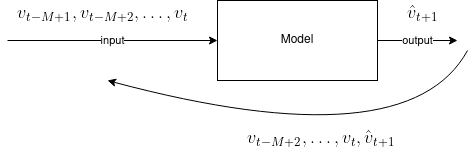
\includegraphics[width=\textwidth]{./images/recursive.png}
  \centering
  \caption{
روش بازگشتی در پیش‌بینی چند گام آینده }
  \label{fig:blocks}
\end{figure}


\قسمت{ابزارها و امکانات مورد نیاز}
مرتبه زمانی روش پیچش روی گراف به این دلیل که امکان استفاده از تبدیل سریع فوریه\پانویس{FFT} وجود ندارد،
\[
O(n^{2})
\]
می‌باشد و اعمال این روش بدون داشتن تجهیزات گران قیمتی مانند پردازنده‌های گرافیکی زمان قابل توجهی است. حداقل امکانات مورد نیاز برای اجرای این پروژه عبارت اند از:

\begin{latin}\begin{itemize}
\item CPU: Intel(R) Xeon(R) CPU E5-2620 v4 @ 2.10GHz
\item GPU: NVIDIA GeForce GTX 1080
\end{itemize}\end{latin}

\قسمت{توضیح دیتاست}
مدل را دوبار به وسیله ی دو داده‌گان متفاوت آموزش دادیم.

\زیرقسمت{داده‌گان \متن‌لاتین{PeMSD7}}

این دیتاست توسط دوربین‌های سرعت‌سنجی که در نقاط مختلف قرار می‌گیرند جمع آوری شده‌اند. محل استقرار این دوربین‌ها ثابت است و کار ما در ساختن ماتریس فاصله بسیار ساده می کند همچنین سرعتی که این دوربین‌ها گزارش می‌دهند بسیار قابل اعتماد است و دیتاستی که با آن کار کردیم نیز داده‌ی پرت و یا گمشده‌ی کمی داشت و همانظور که در جدول \رجوع{} مشاهده می‌کنید مدل آموزش داده شده با این دیتاست دقت بالایی دارد.

\زیرقسمت{داده‌گان \متن‌لاتین{Snapp}}

این دیتاست توسط سیستم موقعیت‌‌یاب‌جهانی رانندگان جمع‌آوری شده‌است در نتیجه نمی‌توان سرعت ترافیک یک نقطه را پیدا کرد بلکه می‌توان
به طور مثال سرعت ترافیک در یک خیابان را دانست این موضوع ساختن ماتریس فاصله را مشکل می‌کند همچنین داده‌های آن به دلایل متعدی مانند
وجود ساختمان‌های بلند قابل اعتماد نیست. همچنین این داده در ابتدا سرعت ترافیک در یک خیابان نیستند بلکه سیگنال‌های \متن‌لاتین{GPS} رانندگان است. برای آماده کردن داده مراحل زیر انجام شده است.

\شروع{شمارش}

\فقره نوشتن \متن‌لاتین{cron job} برای گرفتن داده‌گان: به علت حجم بالای داده‌گان گرفتن تمام داده‌گان به صورت پشت‌سر‌هم مقدور نبود
در نتیجه \متن‌لاتین{cron job} نوشته شد تا در هر دقیقه تلاش کند و یک \متن‌لاتین{bulk} از دادگان را بگیرد.

\فقره نگاشت نقطه بر نقشه\پانویس{map matching}: سیگنال \متن‌لاتین{GPS} رانندگان به صورت دقیق بر روی خیابان نمی‌افتد و ابتدا باید خیابان مربوط به هر سیگنال \متن‌لاتین{‌GPS} را پیدا کنیم.

\شروع{شکل}
  \درج‌تصویر[height=8cm]{./images/mapMatch.png}
  \تنظیم‌ازوسط
  \شرح{نگاشت نقطه بر نقشه}
  \برچسب{fig:time-conv}
\پایان{شکل}

هر سیگنال \متن‌لاتین{GPS} متعلق به یک خیابان است که خیابان مورد نظر برای ما پنهان است و ما تنها سیگنال را می‌توانیم مشاهده کنیم
از طرفی ما رشته‌ی این سیگنال‌های \متن‌لاتین{GPS} را داریم، در نتیجه می‌توانیم از الگوریتم مدل پنهان مارکوف\پانویس{hidden markov model} \مرجع{Rabiner1986} استفاده کنیم.
برای هر سیگنال می توان $k$ خیابان نزدیک به آن را به عنوان حالت‌های پنهان احتمالی فرض کرد و سپس احتمالات انتشار و انتقال را به‌دست‌آورد.

\شروع{شکل}
  \درج‌تصویر[height=8cm]{./images/hmm.png}
  \تنظیم‌ازوسط
  \شرح{مدل پنهان مارکوف}
  \برچسب{fig:time-conv}
\پایان{شکل}

حال با استفاده از الگوریتم ویتربی\پانویس{viterbi} می توانیم محتمل‌ترین رشته و در نتیجه محتمل‌ترین نگاشت را پیدا کنیم.
پس از اتمام عملیات نگاشت می‌توانیم سرعت حرکت راننده، جهت حرکت او و شماره‌ی مرجع خیابان \پانویس{Road Segment ID} را پیدا کنیم.

\فقره محاسبه‌ی سرعت بر اساس سیگنال‌های \متن‌لاتین{GPS}: یکی از اطلاعاتی که سیگنال \متن‌لاتین{GPS} در اختیار ما قرار می‌دهد سرعت است اما این سرعت به صورت لحظه‌ای است و دارای خطای بسیار زیادی است به همین دلیل خود به محاسبه‌ی سرعت می‌پردازیم. پس از مرحله‌ی قبل که رشته‌ی \متن‌لاتین{GPS}های پشت‌سر‌هم به دست آمدند از تقسیم فاصله‌ی کروی دو سیگنال پشت‌سر‌هم بر اختلاف زمانی رخ دادن آن‌ها سرعت محاسبه می‌شود.

\فقره تمیز کردن دادگان: دادگان \متن‌لاتین{GPS} رانندگان دارای صفر و داده‌های پرت بسیاری است و نیاز دارد تا به دقت پیش‌پردازش شود. به طور مثال باید چک شود که دادگان راننده‌ّهایی که در حال سفر نیستند حذف شود.


۴. تمیز کردن دادگان: دادگان /متن‌لاتین{GPS} رانندگان دارای صفر و داده‌های پرت بسیاری است و نیاز دارد تا به دقت پیش‌پردازش شود. به طور مثال باید چک شود که دادگان راننده‌ّهایی که در حال سفر نیستند حذف شود.

۵. حذف داده‌ی غیرقابل اعتماد: هدف در این پروژه ارایه‌ی مدلی بود که بتواند به خوبی سرعت ترافیک را پیش‌بینی کند مساله‌ی مسیریابی در حوزه‌ی کاری این پروژه نمی‌گنجد اما ذکر این موضوع خالی از لطف نیست که حتی اگر مدل ما توانایی بالایی در یادگیری دیتایی که به آن می‌ٔدهیم و پیش‌بینی سرعت ترافیک داشته باشد خطا در گام‌های اولیه مانند محاسبه‌ی سرعت باعث می‌شود دیتاستی که مدل قرار است به وسیله‌ی آن آموزش ببیند دارای نویز زیادی باشد و هدف ایده‌آل ما که مسیریابی است کاملا تحت‌الشعاع قرار می‌گیرد به همین دلیل در مکان‌هایی که دیتای قابل اعتمادی نداریم به طور مثال وقتی تعداد کل سیگنال‌های متن‌لاتین{GPS} که در یک خیابان مشخص در اختیار داریم از آستانه‌ی مشخصی پایین‌تر باشد سرعت آن خیابان را برابر general flow قرار می‌دهیم
\پایان{شمارش}
